\part{Ontwerp}
\label{ontwerp}

%
% Systeemmodel
%

\chapter{Systeemmodel}
\label{ontwerp:systeemmodel}

De eerste stap van het ontwerp was de identificatie van de verschillende deelsystemen, en op welke toestellen die te vinden zijn. Hiertoe hebben we eerst gekeken naar de verschillende taken die het systeem als een geheel moet vervullen. Zo moet het systeem:
\begin{itemize}
\item Voorstellingen weergeven, en gebruikersinvoer verwerken;
\item Toelaten om eenvoudig voorstellingen te wijzigen, zonder veel technische bagage;
\item Voorzien in een gebruiksvriendelijke beheersinterface;
\item Dit alles voldoende robuust uitvoeren.
\end{itemize}

Hiermee konden we de verschillende deelsystemen identificeren. Zo zijn er natuurlijk de kiosken, die instaan voor de weergave van de voorstellingen, en de verwerking van gebruikersinvoer. Om het systeem flexibel te houden, zullen we de kiosken zo inrichten dat zowel de configuratie als de weer te geven voorstellingen zich niet op voorhand op de kiosk bevinden, maar van een centrale server gehaald worden. Diezelfde centrale server kan dan ook voorzien in een beheersinterface, waarbij de status van de verschillende kiosken gevisualiseerd wordt, en de administrator eventueel bepaalde acties kan ondernemen. Al deze functionaliteit zullen we bundelen binnen het specifiek hiervoor ontworpen applicatie-raamwerk, waarvoor we ook een communicatieprotocol zullen moeten definiëren.

In de volgende hoofdstukken gaan we elk van deze deelsystemen, en al wat daar bij hoort, tot in details uitwerken. Zo zullen we ook frequent bestaande technologieën hergebruiken, of net een gerichte keuze maken zodat hergebruik mogelijk wordt. Daarbij gaan we meestal uit van een initiële selectie aan technologieën die gebruikt kan worden om een specifiek doel te bekomen, waarna de selectie uitgedund wordt tot er slechts 1 mogelijkheid overblijft. Het valt op te merken dat we bij dergelijke selectieprocedures steeds een impliciete doch sterke voorkeur stellen voor open technologieën, waarvoor er een gratis, cross-platform en open-source implementatie bestaat. Dat we kiezen voor technologieën met een kosteloze implementatie, vloeit voort uit het beperkte budget dat toegekend is door de MIRA vzw. Het cross-platform aspect is belangrijk omdat op termijn de applicatie misschien op een ander systeem zal moeten draaien, alsook zal het in geval van een succesvol eindproduct de openstelling voor andere bedrijven bevorderen. Het open-source kenmerk tenslotte kent zijn oorsprong weliswaar deels in idealistische gronden, maar blijkt in de praktijk ook zeer praktisch te zijn. Zo is het tijdens de realisatie van het project verschillende keren extreem nuttig gebleken om vrije toegang te hebben tot de broncode van de bibliotheek.


%
% Applicatie
%

\chapter{Applicatie}
\label{ontwerp:applicatie}

In volgende hoofdstuk bespreken we het ontwerp van de applicatie. Daarbij zullen we eerst de technologieën vastleggen, om vervolgens het exacte gebruik ervan te documenteren. Hiertoe hebben we vaak gebruik gemaakt van prototypes: kleine applicaties die gebruik maken van de technologie of bibliotheek in kwestie, om zo op voorhand reeds zicht te hebben op de kwaliteit ervan.

In realiteit was dit proces echter niet zo afgelijnd: vaak leidde een bepaalde beslissing tot het terugkomen op een voorheen gemaakte keuze. In meerdere gevallen zal het dan ook voorkomen dat een specifieke eis uit het niets gegrepen lijkt, of bevooroordeeld schijnt te zijn. Toch is dit niet het geval, pas na afloop van het hoofdstuk zal het totale plaatje duidelijk worden, nadat alle beslissingen mooi in de plooi gevallen zijn.

\section{Voorstellingen}
\label{ontwerp:applicatie:voorstellingen}

\subsection{Formaat}

Aan het formaat van de voorstellingen worden een aantal specifieke eisen gesteld:
\begin{itemize}
\item Terugwaarts compatibel met de huidige voorstellingen;
\item Efficiënt te distribueren over het netwerk;
\item Flexibel en toekomstgericht;
\item Eenvoudig weer te geven;
\item Laagdrempelig.
\end{itemize}

Zoals reeds gezegd bevinden de oude voorstellingen zich op een Dvd-schijf, in videoformaat. Het nieuwe formaat moet dus in staat zijn om video's weer te geven, eventueel na bepaalde conversies (herwerken van alle bestaande media is immers niet haalbaar).

Het eerste idee was dan ook om de reeds digitale \strong{Dvd-bronbestanden te streamen} naar de kiosken. Een eerste probleem met deze opzet is de grootte van de bronbestanden (gemiddeld $3 GB$ per Dvd), wat enerzijds voldoende opslagcapaciteit vereist aan de kant van de server, en het anderzijds moeilijk maakt om het geheel te cachen aan de kant van de kiosk waardoor zowel de server als het netwerk aan een continue belasting zullen onderworpen worden. Die netwerkbelasting is tevens niet van de minste: de Dvd-standaard beschrijft dat de videobestanden een piekbitrate van maar liefst $10 Mb/s$ kunnen hebben, waardoor de server alsook de infrastructuur zouden moeten voorzien in hardware die tot $1 Gb/s$ moet kunnen verwerken.

Om deze problemen op te lossen hebben we gedacht aan het \strong{streamen van gecomprimeerde videobestanden}. Indien we bijvoorbeeld de video comprimeren met de moderne \code{H264} compressiestandaard (getest met de \code{x264} encoder en diens standaard compressieparameters), reduceren we de piekbitrate tot $2.5 Mb/s$ zonder daarbij te moeten inboeten aan kwaliteit. Toch kunnen we dit nog steeds niet efficiënt noemen, vooral omdat eerder statische of zelfs puur tekstuele gegevens nog steeds voorgesteld worden door videogegevens. Ook is het systeem niet flexibel: complexe logica of interactieve voorstellingen kunnen niet of maar heel omslachtig gerealiseerd worden.

Daarom hebben we het over een andere boeg gegooid en gekeken naar \strong{specialistische presentatieformaten}, zoals die van \code{Powerpoint} of \code{OpenDocument Presentation} bestanden. Hierbij is het veel eenvoudiger om complexe en interactieve voorstellingen te realiseren, alsook worden die gegevens efficiënt en flexibel opgeslagen. Ook kunnen we de bestaande videobestanden gebruiken binnen de voorstellingen, afhankelijk van het presentatieformaat door ze erin te verwerken of door te verwijzen naar een extern bestand. Maar ook dit systeem is niet ideaal: weergeven van de bestanden buiten de applicatie waarvoor ze ontwikkeld is om, is niet eenvoudig. Ook is het vervelend dat het eindresultaat bestaat uit een binair bestand, waardoor het bijvoorbeeld niet mogelijk wordt om wijzigingen aan de voorstellingen efficiënt door te sturen.

Om toch de voordelen van speciale presentatieformaten te benutten, zullen we ze implementeren met \strong{\ac{html} en Javascript}, een veelgebruikte combinatie bij het maken van moderne websites. Hierbij is het nog steeds mogelijk om complexe voorstellingen te realiseren, en worden die efficiënt opgeslagen. Alle code wordt immers opgeslagen in tekstformaat, en de ondersteunde video- en audiostandaarden zijn steeds gekozen wegens hun efficiënte netwerkoverdracht. Verder kunnen ook afbeeldingen en video's efficiënt gemaakt worden door ze te realiseren in een vectorformaat\footnote{Afbeeldingen via het \code{<svg>} element, en video's via \code{<canvas>} en Javascript code.}. Ook biedt \ac{html} sinds versie 5 de mogelijkheid om bestaande multimediabestanden weer te geven (via de \code{<video>} en \code{<audio>} tags), waardoor we de terugwaartse compatibiliteit met het huidige systeem bekomen. Ook bestaan er enorm veel Javascript codebibliotheken, waardoor het via hergebruik daarvan mogelijk wordt om zeer dynamische voorstellingen te realiseren. Tenslotte is het ook eenvoudig om dergelijke bestanden weer te geven in een externe applicatie, door gebruik te maken van bestaande rendering engines. Een minpunt is wel de manier waarop de logica geïmplementeerd is: de designer moet steeds een notie van Javascript hebben. Het is wellicht mogelijk om zoveel mogelijk te abstraheren in een externe Javascript bibliotheek, maar toch blijft de scheiding tussen design en code vager dan het is bij de andere systemen. Ook bestaan er (nog) geen bruikbare \ac{wysiwyg} editors, waardoor het steeds nodig is om \ac{html} code, hoe laagdrempelig die ook is, te bewerken.

\begin{table}[h!]
  \begin{center}
    \begin{tabular}{p{3cm} p{4cm} p{4cm}}
    & Dvd-bronbestanden & Compressie\\
    \hline
    Compatibiliteit & Volledig compatibel & Mits conversie \\
    Efficiëntie & Inefficiënt & Inefficiënt \\
    Flexibiliteit & Zeer omslachtig & Zeer omslachtig \\
    Externe weergave & Eenvoudig & Eenvoudig \\
    Complexiteit & Relatief eenvoudig & Relatief eenvoudig \\
    \\    
    & Presentatieformaten & \ac{html} en Javascript \\
    \hline
    Compatibiliteit & Embedden & Embedden na conversie \\
    Efficiëntie & Efficiënt & Zeer efficiënt \\
    Flexibiliteit & Flexibel & Extreem flexibel \\
    Externe weergave & Moeilijk & Relatief eenvoudig \\
    Complexiteit & Zeer eenvoudig & Relatief moeilijk \\
    \end{tabular}
  \end{center}
  \caption{Vergelijking van verschillende formaten.}
\end{table}

Na zorgvuldig afwegen van de voor- en nadelen hebben we gekozen voor de combinatie van \ac{html} en Javascript, aangezien het als enigste systeem voldoet aan alle functionele eisen. Het grote minpunt, de moeilijkheid om voorstellingen te wijzigen wegens de mindere duidelijke scheiding tussen design en code, zal immers verbeteren na verloop van tijd. Zo zullen er wellicht Javascript-bibliotheken ontwikkeld worden om presentatielogica te abstraheren, en kan het best zijn dat er binnenkort betere \ac{wysiwyg}-editors voor moderne \ac{html} boven water komen.

\subsection{Repository}

Zoals hierboven reeds vermeld, zullen noch de nieuwste voorstellingen noch de configuratie zich direct op de relevante kiosken bevinden, maar dynamisch van de centrale server gedownload worden. Indien voorzien wordt in een gebruiksvriendelijk systeem om de media te wijzigen, maakt dit het leven van de administrator ook een pak gemakkelijker nu hij niet meer moet deployen naar elke kiosk apart.

Initieel zijn we op zoek gegaan naar een \strong{database-systeem} om dit te implementeren. Hoewel dergelijke systemen vooral sterk zijn in het herbergen van gestructureerde data, zou het perfect mogelijk zijn om er de eerder bestandsgeoriënteerde voorstellingen in op te slaan. Efficiënte overdracht wordt echter niet voorzien, en bovendien zou het vrij moeilijk zijn om een gebruiksvriendelijke interface te bouwen bovenop dit systeem.

Een andere verzameling technologieën die we overwogen hebben, waren de \strong{Enterprise Content Management} systemen. Hierbij vinden we al vaker een geïntegreerde beheersinterface, alsook komt het frequent voor dat een reeds aanwezig versiebeheer-systeem zorgt voor efficiënte dataoverdracht. Toch voldeed deze oplossing niet, daar bij dergelijke systemen de nadruk vaak nog explicieter ligt op gestructureerde data, waardoor het niet praktisch zou zijn om er onze ongestructureerde voorstellingen in op te slaan.

Daarom hebben we uiteindelijk te stap gemaakt naar speciale \strong{versiebeheer-systemen}. Hierbij is efficiënte overdracht van gegevens een basiseigenschap, en zorgt het bestandsgeoriënteerde aspect tegelijkertijd voor een relatief gebruiksvriendelijke interface. Zo kan een administrator heel gemakkelijk lokaal enkele wijzigingen doorvoeren aan een voorstelling, het resultaat testen in zijn browser, en indien gewenst zijn werk doorsturen naar de centrale server. Ook zorgt het ervoor dat het in eerste instantie niet nodig is om te voorzien in een gebruiksinterface maar blijft het wel nog steeds mogelijk om dit later te doen.

Maar er bestaan tientallen versiebeheersystemen, die we elk gepeild hebben aan ons eisenpakket:
\begin{itemize}
\item Client-server georiënteerd;
\item Client-side aspect efficiënt te gebruiken vanuit een applicatie;
\item Server-side aspect liefst ook te integreren binnen een andere applicatie;
\item Efficiënte omgang met binaire bestanden.
\end{itemize}

Er zijn maar weinig versiebeheersystemen die aan dit eisenpakket voldoen. Meer nog, na een uitgebreide vergelijking, blijkt enkel \ac{svn} een geschikte keuze te zijn. Dit ondertussen ruim 10 jaar oud project biedt ons een zeer goed ontwikkeld en stabiel versiebeheersysteem om onze repository mee te realiseren. Ook voorziet het project in een uitgebreide library die toelaat om de repository direct te manipuleren vanuit een externe applicatie. Hierdoor zal relatief eenvoudig zijn om vanuit de client- en serverapplicatie bestanden op te vragen uit de repository, door gebruik te maken van de clientside-bindings in de \ac{svn} bibliotheek. Ook wouden we voor de serverapplicatie een nog hechtere integratie realiseren, waarbij de repository zich eigenlijk binnen de applicatie zou bevinden. Dit zou als voordeel gehad hebben dat we niet zouden moeten berusten op een externe \ac{svn} instantie, maar zoals later zal blijken hebben we uiteindelijk dit idee moeten opgeven.

\subsubsection{Layout}

Hoewel het nu bepaald is dat we een bestandsgeoriënteerde \ac{svn}-repository zullen gebruiken, ligt de exacte layout van de bestanden daarin nog niet vast. Aangezien zowel de voorstellingen als de kioskconfiguratie erin zal moeten opgeslagen worden, is het belangrijk om op voorhand een eenduidige structuur vast te leggen die tevens toelaat om eenvoudig wijzigingen te detecteren.

\begin{lstlisting}[float, caption=Voorbeeld van een repository layout.]
+-repository/
  |
  +-configurations/
  | |
  | +-kiosk1.xml
  | |
  | +-kiosk2.xml
  |
  +-media/
    |
    +-presentation1/
      |
      +-index.html
\end{lstlisting}

Op het hoogste niveau zal de repository bestaan uit twee mappen. In de \code{configurations} map bevinden zich bestanden die een configuratie typeren, elk uniek geïdentificeerd door hun bestandsnaam. De configuratie bepaalt volledig hoe een kiosk zich zal gedragen, zoals welke media ingeladen moet worden of hoe sterk het volume moet staan. Om de implementatie eenvoudig te houden hebben we ervoor gekozen om een een configuratie eenduidig te laten overeenkomen met een enkele kiosk, en niet te voorzien in functionaliteit om gedeelde instellingen weg te abstraheren. Natuurlijk laat het formaat toe om dit in een later stadium toe te voegen.

De \code{media} map bevat de effectieve voorstellingen, elk in een aparte subfolder. Hierin staan de bestanden nodig om de voorstelling weer te geven, waarbij slechts 1 bestand echt vereist is: \code{index.html}. Dit bestand is de entrypoint in de voorstelling, en zal door de client ingeladen worden wanneer de presentatie moet weergegeven worden. Het zou natuurlijk mogelijk zijn om dit op een flexibelere manier op te lossen, bijvoorbeeld via een extra configuratie bestand, maar opnieuw kiezen we ervoor om initieel een eenvoudig maar compleet raamwerk te voorzien en pas in een later stadium eventueel te voorzien in extra features.

\paragraph{Bestandsformaat}

Bij de voorstellingen is het reeds duidelijk welk formaat de bestanden moeten hebben, namelijk geldige HTML code. Bij de configuratiebestanden daarentegen moeten we zelf nog op zoek gaan naar een gepast formaat om de informatie in op te slaan. Hierbij zullen we opnieuw eerst bepalen wat onze eisen zijn:
\begin{itemize}
  \item Eenvoudig te bewerken;
  \item In te laden vanuit een externe applicatie, zonder daarbij al te veel werk te moeten verrichten;
  \item Correctheid moet te verifiëren vallen.
\end{itemize}

Als eerste kandidaat hebben we gekeken naar het \strong{INI formaat}, een populair \code{key=value} formaat dat zijn origines kent binnen oudere Windows versies. Hoewel dit eigenlijk helemaal geen krachtig en zeker geen eenvoudig te verwerken formaat is, leek het interessant omdat het eenvoudig te bewerken en relatief intuïtief is. Ook zijn er veel bibliotheken beschikbaar om dergelijke bestanden in te lezen, al moet het gezegd zijn dat het voor zo een eenvoudig formaat eigenlijk helemaal niet nodig is om op zoek te gaan naar een gedediceerde biblitoheek.

Van zodra we echter begonnen aan de effectieve implementatie van de applicaties, bleek het formaat niet voldoende voor onze toepassing. Zo hadden we op een gegeven moment nood aan een hierarchische datastructuur, wat bij een ini-bestand onmogelijk is. Ook hebben we een tijdje last gehad van een bug die veroorzaakt werd door een typfout in een configuratiebestand, iets dat de parser niet merktte bij gebrek aan verificatiemogelijkheden. Daarom hebben we besloten om op zoek te gaan naar een alternatief, dat we gevonden hebben onder de vorm van \strong{\ac{xml} bestanden}. Dit formaat kent enkele duidelijke voordelen: zo is het enerzijds mogelijk om hierarchische datastructuren te modelleren, en bestaan er verschillende mechanismen om de bestanden te verifiëren vooraleer ze effectief in te laden. Voor dat laatste zullen we kiezen voor \ac{xml} schema, waartoe we eerst een \ac{xsd} bestand zullen moeten maken dat het exacte formaat van de configuratiebestanden formeel beschrijft. Ook bestaan er talloze bibliotheken om de bestanden in code in te laden. Toch kent het formaat een belangrijk nadeel: het is nu niet meer zo gebruiksvriendelijk om het met de hand te bewerken. Daartoe zullen we in de toekomst misschien een kleine applicatie ontwerpen die een administrator toelaat om een kiosk te configureren via een gebruiksvriendelijke wizard, waarbij deze applicatie handig gebruik zal kunnen maken van het \ac{xsd} bestand. 

\begin{lstlisting}[language=XML, float, caption=Voorbeeld van een kiosk configuratiebstand, label=code:kioskconfiguratie]
<?xml version="1.0"?>
<kiosk xmlns="http://www.mira.be">
  <target>0026b900-926f-1000-8000-000000000000</target>
  <device>
    <sound>
      <volume>255</volume>
    </sound>
  </device>
  <application>
    <media id="manen" />
  </application>
</kiosk>
\end{lstlisting}

De specificatie van de \ac{xml} bestanden is zodanig gemaakt dat het eenvoudig te mappen valt over de services waarmee de server een kiosk kan controleren (zie later).

\subsubsection{Verwerking}

Nu de gegevens binnen de repository gesplitst zijn in twee delen, de configuraties en de voorstellingen, valt het nog te bepalen wie instaat voor de verwerking van welke gegevens. Betreffende de \strong{voorstellingen} is het eenvoudig om te zien dat we best de client hiervoor verantwoordelijk stellen. Als we immers de server zouden laten instaan voor het ophalen van de media, dan zouden we zelf moeten zorgen voor het efficiënt overdragen van de gegevens naar de client. Als we echter vanuit de client rechtstreeks contact opnemen met de repository maken we gebruik van de jaren na jaren aan optimalisaties en verbeteringen doorgevoerd aan het \ac{svn} protocol.

Betreffende de \strong{configuraties} is het een complexere afweging. Moesten we de configuraties laten verwerken door de clients, dan zouden we maar op 1 plek contact opnemen met de repository, wat natuurlijk de beste oplossing lijkt. Toch hebben we ervoor gekozen om de configuraties door de server te laten inlezen, wat essentieel twee grote nadelen heeft: de serverapplicatie vereist er een clientside \ac{svn} library door, en op de clients zullen we de nodige interfaces moeten voorzien om configuratie over het netwerk toe te laten. De motivatie voor deze keuze was als volgt:

\begin{enumerate}
\item Vooreerst is er het probleem van monitoring. Aangezien een beheerder op elk moment wijzigingen kan uploaden, moet de partij die verantwoordelijk is voor het ophalen van gegevens periodiek de repository controleren. Als we hiervoor de client zouden gebruiken, betekent dit dat een potentieel groot aantal clients periodiek contact opneemt met de server, wat niet echt efficiënt is. Ook is er het probleem van scheduling: als elke client volledig onafhankelijk de repository in de gaten houdt en ageert wanneer wijzigingen plaatsvinden, is het onmogelijk om extreme belasting van de server te vermijden door de clients slechts sequentieel toegang tot de repository te verlenen. Het is dus duidelijk dat we binnen de server sowieso een clientside \ac{svn} library zullen moeten voorzien.
\item Een tweede motivatie is de nood aan een krachtige configuratie-tool. Een administrator moet de mogelijkheid hebben om via een tool (hetzij een webinterface, hetzij een lokale applicatie) direct een actie teweeg te brengen op een kiosk naar keuze. Het kan bijvoorbeeld zijn dat een kiosk afgesloten moet worden, of dat heel snel al het geluid moet afgezet worden. Het is logisch dat dit buiten de repository om moet kunnen, en om dit te realiseren moeten de client-applicaties voorzien in een bepaalde interface die toelaat om acties teweeg te brengen.
\end{enumerate}

Het is dus duidelijk dat het geen extra complexiteit teweegbrengt om de configuraties binnen de serverapplicatie te verwerken (zowel een clientside \ac{svn} library als de nodige configuratieinterfaces zijn sowieso nodig), meer nog, het is een interessante oplossing omdat we zo tenminste de belasting van de server kunnen controleren door het updaten van de clients intelligent te schedulen.

\section{Netwerk}
\label{ontwerp:applicatie:netwerk}

De verschillende onderdelen van het systeem zullen niet enkel lokaal werken, maar ook met elkaar communiceren over het netwerk. Zo zullen de voorstellingen, waarvan we het formaat en reeds vastgelegd hebben, via het netwerk naar de kiosken overgedragen worden. Maar ook het beheer zal over het netwerk verlopen: via een centrale beheersapplicatie kan een werknemer de status van de kiosken te bekijken, en eventueel bepaalde acties te ondernemen. Die acties worden daarbij niet beperkt tot louter beheerstaken: om het geheel eenvoudig te houden zal hetzelfde mechanisme ook gebruikt worden om essentiële applicatiefunctionaliteit (zoals het inladen van een voorstelling, of het doorvoeren van de instellingen die de ingeladen configuratie vereist) te realiseren.

\subsection{Dataoverdracht}

Aangezien we gebruik maken van een losstaand versiebeheersysteem (zie \ref{ontwerp:applicatie:voorstellingen}), namelijk \ac{svn}, zullen we ook gebruik maken van diens dataoverdrachtmogelijkheden.

\subsection{Netwerkconfiguratie}

Om het systeem eenvoudig in gebruik te maken, hebben we er voor geopperd om zoveel mogelijk configuratie automatisch te laten verlopen. Er blijft echter steeds één link die manueel moet gelegd worden: namelijk welke voorstelling naar elke kiosk moet gestuurd worden. Hoe we de overige configuratie automatiseren wordt besproken in de volgende paragrafen.

\subsubsection{Discovery}

Service discovery staat in voor het publiceren van en luisteren naar meldingen waarbij een toestel zijn diensten adverteert op een bepaald netwerkkanaal. Hierbij wordt vaak aangegeven wat de naam is van het toestel, en wat de exacte mogelijkheden zijn van elke dienst. Zoals duidelijk is gaat dit hand in hand met het aspect van naamresolutie: hoe moet een luisterende partij contact opnemen met het toestel dat zonet zijn diensten geadverteerd heeft. Omdat beide aspecten vaak aangepakt worden via eenzelfde mechanisme, behandelen we ze ook samen in een enkele paragraaf.

Zoals zo vaak het geval is, bestaan er verschillende technologieën die voorzien in dergelijke functionaliteit. Om een selectie te kunnen maken, stellen we enkele bijkomende eisen: 
\begin{itemize}
\item Vereist geen extra infrastructuur;
\item Cross-language implementatie;
\item Robuust en stabiel.
\end{itemize}

Een veelgebruikt protocol voor service discovery, is het \strong{\ac{ssdp}}, deel van het \ac{upnp} systeem. Dit door Microsoft-ontwikkeld systeem, biedt een heel uitgebreid en generisch raamwerk voor service discovery, waarbij die services volledig beschreven worden door het \ac{dcp}. Het geheel steunt sterk op XML en SOAP, en is strikt beheerd door het \ac{upnp} Forum. Hoewel het protocol essentieel wel voldoet aan onze eisen, is het niet zo eenvoudig in gebruik en biedt het veel te veel mogelijkheden die we toch niet gaan gebruiken.

Een compacter alternatief is \strong{\ac{mdns}}, onderdeel van het door Apple ontwikkelde Zeroconf systeem. Zoals de naam doet vermoeden, is dit een multicast uitbreiding van het \ac{dns}, dat de \code{SRV} records gebruikt om services te publiceren. Dit is een veel eleganter systeem, essentieel slechts een eenvoudige uitbreiding van een bestaande technologie, maar kent zo ook zijn tekortkomingen. Zo worden bijvoorbeeld de mogelijkheden van elke service gedetailleerd via een verder niet gespecificeerd tekstveld. Dergelijke tekortkomingen zijn echter niet van belang in de context van dit systeem, waardoor het min of meer evenwaardig is met \ac{ssdp}.

Wegens de eenvoud elegantie van het protocol, was de initiële implementatie dan ook gebaseerd op \ac{mdns} door gebruik te maken van de \code{JmDNS} bibliotheek. Na verloop van tijd bleek die bibliotheek echter niet zo stabiel: zo kwam het soms voor dat een kiosk die zichzelf gepubliceerd werd, niet door de server herkend werd. Aangezien dergelijke stabiliteitsproblemen totaal onaanvaardbaar zijn, en \code{JmDNS} de enige \ac{mdns} implementatie voor Java is (platformgebonden code hierbij niet in achting genomen), hebben we uiteindelijk moeten overschakelen naar \ac{upnp}.

\subsubsection{Adressering}

Hoewel we nu beschikken over een systeem dat zonder enige configuratie toelaat om een kiosk te vinden en contacteren, is er nog steeds nood aan een mechanisme die de netwerkinterfaces op de kiosken configureert. Maar omdat elk contact volledig dynamisch verloopt, maakt het eigenlijk niet uit welke adressen toegewezen worden aan individuele kiosken, de enige vereiste is dat de adressen legaal zijn waardoor netwerkcommunicatie correct kan verlopen.

De meest logische keuze hiervoor is het \ac{dhcp} protocol, een veelgebruikt en robuust protocol waarbij de kiosken bij het opstarten een aanvraag voor een adres broadcasten. Hierbij wordt rekening gehouden met welke adressen reeds ingenomen zijn, waardoor er geen conflicten zullen optreden bij het toewijzen van adressen. Een nadeel aan \ac{dhcp} is dat het nood heeft aan een serverapplicatie die instaat voor het uitdelen en beheren van adressen, maar aangezien we toch een router zullen nodig hebben binnen het netwerk en quasi elke router een \ac{dhcp} server aan boord heeft, vormt dit niet echt een probleem.

Een toekomstgericht alternatief dat we misschien in een volgende versie zouden kunnen implementeren, maakt gebruik van \ac{ip} versie 6, terwijl we voor de huidige setup kiezen voor \ac{ip} versie 4. Versie 6 kent immers een robuustere en snellere vorm van local-link adressering, waardoor het mogelijk zou zijn om de kiosken zichzelf volledig autonoom een adres te laten toekennen.

\subsection{Controle}

In eerste instantie, toen we er nog van uitgingen dat we geen \ac{upnp} zouden gebruiken, zijn we op zoek gegaan naar eenvoudige \emph{remote procedure} protocollen om zo zonder teveel overhead de nodige acties op de kiosken te kunnen teweegbrengen. In die categorie vinden we zo \strong{\ac{rest}}. Hoewel dit lichtgewicht, \ac{http}-gebaseerd, en ook veelgebruikt protocol op het eerste zicht aan onze eisen voldoet, kent het zijn mindere kanten. Zo kent het geen eenduidige manier om fouten terug te geven, alsook is het formaat waarin gegevens verstuurd worden niet gestandaardiseerd. Omdat de implementatie daarvan nog vrij veel werk zou vereisen, besteden we verder geen aandacht aan dit protocol.

De meest courante ontwikkelframeworks zoals .NET en Java kennen meestal ook hun eigen \ac{rpc}-protocol, zoals \strong{.NET Remoting} en \strong{\ac{rmi}}. Hoewel deze protocollen meestal goed doorontwikkeld en veelzijdig zijn, kunnen ze vaak maar op een enkel platform gebruikt worden en zijn ze al zeker niet cross-language.

Ook hebben we meer moderne \ac{rpc}-frameworks overwogen zoals \strong{Apache Etch}, of \strong{Apache Thrift}. Deze vrij nieuwe en tevens veelbelovende systemen bleken echter enkele kritieke eisen mis te lopen. Zo kent Apache Etch slechts weinig language bindings, en kent geen van beide een authenticatiemechanisme.

Vervolgens hebben we de nodige aandacht besteed aan \strong{XML-RPC}, een zeer simplistisch \ac{rpc}-protocol dat XML-geformatteerde berichten verstuurt over \ac{http}. Jammer genoeg kent XML-RPC enkele fundamentele problemen, zoals het inefficiënte berichtformaat. Ook is de specificatie, om het zacht uit te drukken, vrij beperkt. Dit kan echter een voordeel zijn: de ermee geïmplementeerde interface wordt er compact mee gehouden, en valt eenvoudig te gebruiken vanuit verschillende talen. Dit wordt verder vereenvoudigd door het groot aantal implementaties, voor de meeste talen zijn er verschillende te vinden.

Van zodra we echter het service discovery mechanisme overgezet hebben naar \ac{ssdp}, hebben we besloten om ook voor de acties gebruik te maken van \strong{\ac{upnp}}, dat de mogelijkheid biedt om bij het adverteren van een toestel te voorzien in verschillende \emph{services} en een exacte beschrijving van de verschillende acties die via die service kunnen ondernomen worden.

\subsection{Device en service descriptions}

Om een \ac{upnp} client na het ontdekken van een toestel en diens services toe te laten om het toestel ook effectief te controleren, heeft de client meer informatie nodig. Zo zal de client een \strong{device description} kunnenn opvragen, waarin informatie staat die het toestel identificeert en gedeeltelijk beschrijft. Ook zullen we voor elk van zijn services moeten voorzien in een \strong{service description}. Beide zijn steeds opgemaakt als een \ac{xml} bestand, met de opmaak gedicteerd door de \ac{upnp} specificatie. Bij veel libraries moeten we echter nooit zelf de bestanden schrijven, maar worden ze gegenereerd via een hulpklasse of (zoals vaak het geval is bij libraries voor dynamische talen) worden ze via introspectie afgeleid van een relevante klasse.

\subsubsection{Device description}

Om ons toestel te laten voldoen aan de \ac{upnp} specificatie voorzien we in de volgende gegevens:

\begin{table}[h!]
  \begin{center}
    \begin{tabular}{r l}
    \hline
    Type & \texttt{urn:mira-be:device:Kiosk:1} \\
    Friendly name & Multimedia kiosk \\
    Manufacturer & Volkssterrenwacht MIRA vzw \\
    Manufacturer URL & www.mira.be \\
    Model description & Flexible network-enabled multimedia kiosk \\
    Model name & Ad-Astra Kiosk \\
    Model number & 3.0 \\
    Model URL & https://sites.google.com/site/miraadastraiii/ \\
    Serial number & 1.0 \\
    \hline
    \end{tabular}
  \end{center}
  \caption{Velden binnen de \ac{upnp} device description.}
\end{table}

Naast deze statische gegevens zullen we ook moeten voorzien in een unieke identifier die het toestel identificeert binnen het netwerk. Dit zullen we bespreken bij de effectieve implementatie van de kiosk.

\subsubsection{Service description}

Aangezien deze taak zal verzorgd worden door een applicatie geschreven in C++ (de motivaties hiervan worden later beschreven) is het moeilijker om de service description bestanden dynamisch te genereren. Meer nog, voor de library die we zullen gebruiken zullen we de description files manueel moeten uitschrijven. Hoewel niet zeer arbeidsintensief, is het een foutgevoelig proces dat we liefst niet teveel willen doen. Daarom hebben we eerst grondig nagedacht over hoe de service er moet uitzien, om pas daarna over te gaan tot de effectieve implementatie. Hoewel we nog altijd af en toe wijzigingen hebben moeten doorvoeren aan de service description files, is dit hierdoor tot een minimum beperkt gebleven.

\paragraph{Functionele opdeling}

Om een overvloed aan functies binnen een enkele service te vermijden, hebben we ervoor gekozen om een functionele opdeling door te voeren. Zo hebben we de service die toelaat om het toestel te controleren, met functies zoals \code{Shutdown} en \code{SetVolume}. Een tweede service staat vervolgens in voor acties die een impact hebben op de applicatie, zoals \code{LoadMedia}. Een bijkomend voordeel van deze scheiding is dat alle platform- of hardwareafhankelijke code geïsoleerd is binnen een enkele service, wat de implementatie ervan vereenvoudigt.

\begin{table}[h!]
  \begin{center}
    \begin{tabular}{p{4,5cm} p{5cm}}
    \multicolumn{2}{c}{\strong{Device service}} \\
    \hline
    \hline
    Functie & Beschrijving \\
    \hline
    \code{void Shutdown()} & Toestel afsluiten. \\
    \code{void Reboot()} & Toestel heropstarten. \\
    \code{void SetVolume(uint)} & Volume instellen. \\
    \code{uint GetVolume()} & Volume ophalen. \\
    \\
    \multicolumn{2}{c}{\strong{Application service}} \\
    \hline
    \hline
    Functie & Beschrijving \\
    \hline
    \code{void LoadMedia(string)} & Presentatie inladen. \\
    \end{tabular}
  \end{center}
  \caption{Enkele functies uit beide services.}
\end{table}

\paragraph{Description bestanden}

Zoals reeds gezegd zijn dit \ac{xml} bestanden die elk een service tot in alle details beschrijven. De exacte velden in deze bestanden worden opgelegd door de \ac{upnp} standaard, waardoor we ons soms in vreemde moeten wringen om toch een volledig compatibele service te bekomen. Strikte compatibiliteit is hierbij een vereiste omdat een van de libraries die we zullen gebruiken erop staat dat elk toestel volledig voldoet aan de \ac{upnp} specificatie. Een consequentie hiervan is bijvoorbeeld dat elke parameter van een functie moet overeen komen met een \code{state variable}, ook al heeft dat soms niet echt een praktisch nut.

\begin{lstlisting}[language=XML, float, caption=Voorbeeld van een service descriptor]
<?xml version="1.0"?>
<scpd xmlns="urn:schemas-upnp-org:service-1-0">
  <specVersion>
    <major>1</major>
    <minor>0</minor>
  </specVersion>
  <actionList>
    <action>
      <name>Shutdown</name>
    </action>
    <action>
      <name>SetVolume</name>
      <argumentList>
        <argument>
          <name>iVolumeValue</name>
          <relatedStateVariable>Volume</relatedStateVariable>
          <direction>in</direction>
        </argument>
      </argumentList>
    </action>
  </actionList>
  <serviceStateTable>
    <stateVariable sendEvents="no">
      <name>Volume</name>
      <dataType>ui1</dataType>
      <defaultValue>0</defaultValue>
    </stateVariable>
  </serviceStateTable>
</scpd>
\end{lstlisting}

\subsection{Presentatie}

De \ac{upnp} standaard voorziet tenslotte ook nog in een presentatie gedeelte, dat omschrijft dat een library kan voorzien in een webpagina waarmee een administrator eenvoudig de status van een device kan bekijken en eventueel acties uitvoeren. We hebben er echter voor gekozen dit niet te gebruiken, daar dit zou vereisen dat een administrator manueel surft naar de presentation URL's van elk device dat hij wil beheren. Het alternatief waarvoor we gekozen hebben is een webinterface aan de kant van de server, waarbij acties daar teweeggebracht door de serverapplicatie doorgestuurd worden naar de correcte kiosk.

\section{Redundantie en robuustheid}
\label{sec:redundantie}

Een belangrijk aspect van het systeem is dat het robuust is, en dus voorziet in een bepaalde vorm van redundantie. Zoals het hardwareontwerp zal verduidelijken (zie hoofdstuk \ref{ontwerp:hardware}), voorzien we reeds in hardwarematige redundantie onder de vorm van een RAID configuratie. Toch verhelpt dit het fundamentele probleem niet: de centrale server is een \emph{single point of failure}.

Een eerste idee om dit te verhelpen was het voorzien van een \strong{backup server}, die de centrale server continu zou monitoren. In geval van diens falen, zou de failover functionaliteit geactiveerd worden, waarbij de taken van de centrale server integraal overgenomen zouden worden. Gezien het configuratieloze aspect van de opstelling, en het feit dat elk initiatief steeds van de servers uit komt, zou dit totaal geen actie vereisen. Om ervoor te zorgen dat de backup server steeds over de meest recente informatie beschikt, activeert die tevens een (passieve) \ac{mdns} module, alsook registreert die zich bij de primaire server zodat updates aan de presentatie-repository steeds op beide servers aanwezig zijn.
Hoewel deze configuratie zeer elegant lijkt (zeker indien de replicatie alsook promotie/degradatie van de server volledig autonoom verloopt), is ze niet realistisch op budgettair vlak. Het is niet alleen kostelijk om een tweede voldoende krachtige server samen te stellen, maar de aanwezigheid ervan betekent een extra continue energieconsumptie.

Daarom hebben we gekozen voor een tweede piste, namelijk het gebruik van een \strong{backup-cache in de kiosken}. Aangezien embedded hardware vaak komt met een optie voor een kaartslot, is het voordeliger om voor elke kiosk een dergelijke geheugenkaart aan te kopen. De applicatie zal dan alle opgevraagde voorstellingen en configuratiegegevens lokaal opslaan. Wanneer vervolgens de centrale server onbereikbaar blijkt te zijn, kan steeds gebruik gemaakt worden van deze lokale cache om toch volwaardig te kunnen blijven functioneren.

\section{Server}
\label{ontwerp:applicatie:server}

Zoals reeds vermeld, is de centrale server van essentieel belang in het systeem. Zo verzorgt de server:
\begin{itemize}
\item Configuratie van de kiosken;
\item Opslag en distributie van de voorstellingen.
\end{itemize}

Naast deze elementaire taken, vereenvoudigt de server tevens de werklast van een administrator. We zullen immers voorzien in een beheersinterface die niet alleen een overzicht van het systeem biedt, maar ook toelaat om acties te ondernemen om eventuele problemen te verhelpen.

\subsection{Ontwikkelplatform}

De keuze van het ontwikkelplatform waarvoor we de serverapplicatie zullen ontwikkelen, is van vrij groot belang. Een goede keuze vereenvoudigt en versnelt de ontwikkeling, terwijl een verkeerde keuze tevens de kwaliteit van het eindproduct nadelig kan beïnvloeden.

Opnieuw bestaan er verschillende mogelijkheden die ons essentieel de middelen aanbieden om deze taak te volbrengen. Om een beslissing te kunnen maken, hebben we ons gefocust op de meestgebruikte entiteiten in de wereld van serverapplicaties, namelijk .NET en Java. Hoewel beide kandidaten relatief evenwaardig zijn in de context van deze serverapplicatie, hebben we voor het gemak gekozen voor ontwikkeling in Java. Deze keuze is gemotiveerd door voorgaande ervaringen, maar ook door het feit dat we een voorkeur hebben voor een Linux-gebaseerde omgeving en .NET daar niet goed met samenwerkt.

\subsection{Hergebruik}

\subsection{Repository}

De originele opzet was om via de serverside-bindings in de \ac{svn} bibliotheek te voorzien in een \ac{svn}-compatibele repository die volledig overkoepeld zou zijn door de serverapplicatie. Hierdoor zou het geheel een enkel monolitisch geheel vormen dat geen extra configuratie zou vereisen en niet zou berusten op externe applicaties. Om niet te moeten interfacen met de C-library zouden we daarvoor gebruik maken van de enige Java-wrapper voor de serverside-bindings die er bestaat: \makeurl{http://code.google.com/p/svnj/}{SVN-J}. Jammer genoeg bleek deze library niet stabiel genoeg te zijn, en ontbraken er verschillende features. Daarom hebben we jammer genoeg moeten kiezen voor een externe \ac{svn} repository, niet overkoepeld door de serverapplicatie.

Maar dat is niet alles: een externe \ac{svn} instantie moet altijd overkoepeld worden door een webserver, zoals Apache. Hierdoor zitten we nu met twee webservers: enerzijds Apache, en anderszijds de servlet engine binnen onze serverapplicatie. Om toch enige redundantie te vermijden zullen we Apache gebruiken om onze serverapplicatie te overkoepelen. Dit heeft verschillende voordelen: voor beide servers kunnen we nu de standaardpoort 80 gebruiken, alsook zal het in een later stadium eenvoudiger zijn om hier eventueel een authenticatie- of verificatiesysteem aan toe te voegen. Om de binding tussen Apache en Tomcat te bekomen, zullen we gebruik maken van \code{mod\_jk}, de officiële \makeurl{https://tomcat.apache.org/connectors-doc/}{Apache Tomcat connector}. Hierbij verloopt de communicatie tussen beide over het binaire \ac{ajp} protocol.

\subsubsection{Netwerk}

Tijdens het ontwerp van het applicatieprotocol hebben we er speciaal op gelet om zoveel mogelijk bestaande technologieën te gebruiken, zodat we enerzijds niet steeds het wiel opnieuw uitvinden en anderzijds ook tijdens de realisatie gebruik zouden kunnen maken van bestaande hoogwaardige codebibliotheken.

\paragraph{Configuratie en invocatie} Zoals vermeld verloopt zowel het gros van de netwerkconfiguratie alsook het uitvoeren van acties via \ac{upnp}, wat we uit Java kunnen gebruiken door middel van de \makeurl{http://teleal.org/projects/cling/}{Cling} bibliotheek. Dit is een vrij volledige \ac{upnp} stack die de nadruk legt op strikte conformiteit en een duidelijke API. Hoewel er nog andere \ac{upnp} bibliotheken bestaan, zijn die vaak niet doorontwikkeld, proprietair of niet uitgebreid genoeg, waardoor Cling uiteindelijk de beste keus leek.

\paragraph{Data uitwisseling} Door gebruik te maken van een externe \ac{svn} instantie worden we geconfronteerd met nog een probleem: waar we anders vanuit de serverapplicatie toegang zouden gehad hebben tot de bestanden in de repository (die vervolgens via een \ac{svn}-compatibele interface zouden geopend worden naar eventuele clients toe), moeten we nu zelf contact opnemen met de externe \ac{svn} instantie om de nodige configuratiegegevens op te halen. Ook moet het mogelijk zijn snel te kijken wat de laatste revisie van de repository is, en om vervolgens op te halen wat er veranderd is sinds de laatst bekende revisie. Met die informatie kan bepaald worden welke configuraties en/of voorstellingen opnieuw moeten opgehaald worden, om daarna die informatie door te sturen naar de relevante kiosken.

Hoewel er opnieuw verschillende \ac{svn} bibliotheken bestaan, lijkt \makeurl{http://svnkit.com/}{SVNKit} de enige die nog doorontwikkeld wordt. Ook is de bibliotheek geschreven in pure Java, wat opnieuw het geheel platformonafhankelijk maakt.

\subsubsection{Beheersinterface}

\paragraph{Servlet engine} Om een website te kunnen realiseren, hebben we nood aan een servlet-engine. Binnen de Javawereld zijn er verschillende servlet engines, de bekendste wellicht Tomcat en Jetty. Aangezien onze applicatie niet draait rond de webapplicatie, maar dat slechts een deelcomponent is, zullen we geen gebruik kunnen maken van de standaard servlet environment. Door de servlet engine te \emph{embedden} binnen onze applicatie, is het eenvoudiger om tegelijk verschillende andere niet-webgeoriënteerde services actief te hebben. Zowel Tomcat als Jetty maken het mogelijk om ze te gebruiken binnenin een applicatie, al is het bij de ene al makkelijker dan bij de andere.

We stellen er echter een specifieke eis aan de servlet engine, namelijk dat we bij het genereren van een webpagina tegelijk toegang hebben tot de hele applicatie. Dit vinden we enkel terug bij Tomcat, Jetty start een nieuwe \ac{jvm}. Als we geen speciaal communicatieprotocol zoals \ac{rmi} willen gebruiken om data van de rest van de applicatie op te halen, kunnen we enkel Tomcat gebruiken.

\paragraph{Web tooklit} Nu de servlet engine vast ligt, moeten we nog bepalen met welke technologie we de servlets zullen bouwen. Om ons niet bezig te moeten houden met hoe de webpagina's gegenereerd worden, zijn we op zoek gegaan naar een widget-oriented framework voor moderne webapplicaties. Zo hebben we gekeken naar \strong{\makeurl{http://vaadin.com/home}{vaadin}}, een bibliotheek die toelaat om op een eenvoudige manier met enkel Java code een rijke user-interface te onwerpen. De manier van ontwikkelen leunt nauw aan bij hoe reguliere user-interfaces ontwikkeld worden: event- en widget gebaseerd, zonder zich te moeten bezig houden met het effectief genereren van de interface.

Een probleem met vaadin was echter dat het niet perfect werkt op oudere toestellen, en dat vrij veel code vereiste om een relatief eenvoudige \code{TreeView} op te bouwen. Daarom zijn we eens te meer op onze beslissing teruggekomen, en op zoek gegaan naar een betere toolkit. Zo zijn we gestuit op \strong{\makeurl{http://www.webtoolkit.eu/jwt}{JWt}}. Deze eveneens widget-oriented library heeft een zeer interessante feature, namelijk dat het voorziet in \emph{graceful degradation}. Hierbij zal de library detecteren wat de mogelijkheden zijn van de browser die de pagina opvraagt, en aan de hand daarvan meer of minder gesofisticeerde content genereren. Ook is zijn \ac{api} gemodelleerd naar de Qt \ac{api}, waarmee we reeds ervaring hadden. 

\subsubsection{Logging}

Ook zullen we gebruik maken van het \makeurl{http://logging.apache.org/log4j/1.2/}{Apache log4j} project, om op een uniforme wijze loginformatie te publiceren. Het pakket laat toe om in een extern configuratiebestand te specificeren welke deelmodules hoe gedetailleerd moeten loggen, en wat er met die informatie gedaan moet worden. Zo kunnen we eenvoudig configureren dat kritieke fouten van over heel het systeem moeten doorgemaild worden naar een administrator, of dat een deelsysteem dat nog niet perfect werkt, zoveel mogelijk informatie moet wegschrijven naar een speciaal logbestand.

\section{Kiosk}
\label{ontwerp:applicatie:kiosk}

Naast de server vormen de kiosken het tweede type toestel in het systeem. Een kiosk staat in voor:
\begin{itemize}
\item Weergave van voorstellingen;
\item Verwerken van gebruikersinvoer.
\end{itemize}

\subsection{Ontwikkelplatform}

De keuze van het ontwikkelplatform is eens te meer belangrijk voor het verloop van de ontwikkeling. Nu liggen de eisen echter anders: het platform moet low-level zijn, weinig afhankelijkheden hebben, en toelaten om performante applicaties te realiseren. Opnieuw beschouwen we enkel platformen die werken in combinatie met Linux-gebaseerde besturingssystemen, maar deze keer is de motivatie erachter anders: de meeste embedded hardware ondersteunt enkel een Linux-distributie. Gezien we het aantal afhankelijkheden ook beperkt willen houden, is een geïnterpreteerde taal niet ideaal.

Het ontwikkelplatform \makeurl{http://qt.nokia.com/}{Qt} voldoet vrijwel perfect aan dit eisenpakket. Het platform wordt gebruikt in combinatie met C++, een gecompileerde taal die zeer performante code toelaat. Qt zorgt er echter voor dat ontwikkeling van high-level applicaties zoals deze niet al te arbeidsintensief wordt in het relatief low-level C++. Zo komt Qt met een waaier aan interessante modules om snel een applicatie te realiseren, en breidt het C++ uit met enkele syntactische mogelijkheden die het eenvoudig maken om bepaalde high-level technieken te gebruiken. Bovendien is Qt inherent platform-onafhankelijk, waardoor het mogelijk wordt om de applicatie later eventueel te hergebruiken in een andere omgeving. Tenslotte biedt Qt ook een \emph{embedded mode}, waarin het zelf voorziet in een windowing system. Hierdoor worden enkele zware afhankelijkheden (zoals X11) vermeden.

\subsection{Hergebruik}

\subsubsection{Netwerk}

Net zoals dit bij de serverapplicatie het geval was, kunnen we door de nauwgezette selectie van protocollen optimaal gebruik maken van bestaande bibliotheken.

\paragraph{Configuratie en invocatie} Om een \ac{upnp} bibliotheek te vinden voor C++ moeten we niet lang zoeken. Toch zouden we met een "normale" C++ bibliotheek geen maximale integratie bekomen met de rest van de applicatie. Daarom zijn we specifiek op zoek gegaan naar een \ac{upnp} bibliotheek voor C++, die ook integreert met het Qt framework. Een eerste kandidaat hiervoor is de \makeurl{http://gitorious.org/qupnp}{Qt UPnP} bibliotheek, dewelke poogt een compacte en duidelijke UPnP implementatie te realiseren. Jammer genoeg blijkt dat project nog helemaal niet afgewerkt te zijn, meer nog, verschillende kritieke componenten ontbreken.

Een volgende kandidaat is de \makeurl{http://www.herqq.org/}{Herqq} bibliotheek, opnieuw een Qt-specifieke \ac{upnp} implementatie. De bibliotheek claimt een compacte implementatie conform de specificatie, en een eerste test ervan bleek ook zeer positief te zijn. Initieel zijn we dan ook begonnen met deze bibliotheek, maar hebben we na enkele weken ontwikkeling toch moeten opperen voor een bibliotheek. Het probleem was immers dat niet alleen de \ac{ssdp} configuraties, maar ook de devicegegevens statisch in een \ac{xml} bestand moesten doorgespeeld worden. Hierdoor zou het onmogelijk worden om \emph{at-runtime} een unieke identifier door te geven, waardoor we voor elke kiosk een speciaal configuratiebestand zouden moeten aanreiken. Omdat we uiteindelijk de code volledig generiek willen maken, is dit natuurlijk onaanvaardbaar.

Daarom hebben er uiteindelijk voor gekozen op de C++ \ac{upnp} bibliotheek van het \makeurl{http://brisa.garage.maemo.org/}{BRisa project} te gebruiken. Hoewel het in eerste instantie misschien minder duidelijk was wat de sterktes zijn van deze bibliotheek, maakte een eerste test al snel duidelijk dat ze niet moest onderdoen voor de Herqq \ac{upnp} bibliotheek. Omdat het bij deze bibliotheek wél mogelijk was om dynamisch devicegegevens door te spelen hebben we ervoor gekozen om het te gebruiken binnen de uiteindelijke applicatie.

\paragraph{Data uitwisseling} De kiosk moet in staat zijn een \ac{svn} repository te klonen indien de \ac{webdav} locatie ervan doorgespeeld geweest is. Hoewel we dit best zouden kunnen oplossen door gebruik te maken van de \ac{svn} binary, is dit geen platform-onafhankelijke oplossing, die bovendien niet mooi te integreren valt binnen een applicatie. Daarom zijn we op zoek gegaan naar een C++ bibliotheek, liefst specifiek voor het Qt framework, die ons toelaat gegevens van een \ac{svn} repository binnen te halen zonder daarbij te berusten op een lokaal geïnstalleerde \ac{svn} applicatie. Zo zijn we terecht gekomen bij het \makeurl{http://kdesvn.alwins-world.de/}{KDESvn} project, een KDE frontend voor \ac{svn} repositories. We zijn natuurlijk niet geïnteresseerd in die applicatie, maar in de code die het gebruikt om toegang te krijgen tot \ac{svn} repositories. Daartoe heeft het KDESvn project een bibliotheek ontwikkeld, namelijk \makeurl{http://kdesvn.alwins-world.de/browser/trunk/src/svnqt}{svnqt}. Die bibliotheek is vrijwel volledig losgekoppeld van de KDESvn code, wat integratie binnen andere applicaties eenvoudig maakt (hiervan getuige bijvoorbeeld het \makeurl{http://www.anrichter.net/projects/qsvn}{QSvn} project).

\subsubsection{Weergave voorstellingen}

De voorstellingen zijn opgemaakt in een combinatie van \ac{html} en Javascript. Hierdoor kunnen we voor de weergave gebruik maken van de rendering engines ontwikkeld voor verschillende browsers. Zo is er de \makeurl{https://developer.mozilla.org/en/Gecko}{Gecko} rendering engine, ontwikkeld voor gebruik binnen de producten van Mozilla. Ondanks de recente port van Firefox naar het Qt platform, blijft de integratie van Gecko binnen Qt relatief moeilijk.

Daarom zullen we eerder kiezen voor de \makeurl{http://www.webkit.org/}{WebKit} rendering engine, een doorontwikkeling van de KHTML rendering engine. WebKit is een interessantere keuze gezien zijn populaire port naar het Qt framework, \makeurl{http://trac.webkit.org/wiki/QtWebKit}{QtWebKit}. Deze port is een officieel onderdeel van het Qt framework, waardoor het een goedgedocumenteerd en kwalitatief product is.

\subsubsection{Logging}

Net zoals we bij de serverapplicatie gekozen hebben voor een speciale loggingbibliotheek onder de vorm van log4j, maken we voor deze applicatie gebruik van het vergelijkbare \makeurl{http://log4qt.sourceforge.net/}{Log4Qt}. Dit is een port van log4j naar het Qt platform, zodat het mogelijk is om op een vergelijkbare manier te voorzien in uniforme logging die nauwgezet kan geconfigureerd worden. Omdat het originele project al enige tijd inactief is, zullen we wel gebruik maken van een meer actief ontwikkelde \makeurl{http://gitorious.org/log4qt}{fork} van Log4Qt. De fork is een doorontwikkeling van het originele project, met enkele bijkomend features en bugfixes.


%
% Hardware
%

\chapter{Hardware}
\label{ontwerp:hardware}

Gezien het beperkte budget is de zoektocht naar gepaste hardware best een uitdaging geweest.

\section{Kiosk}
\label{ontwerp:hardware:kiosk}

Algemeen worden er enkele vrij zware eisen gesteld aan de kioskhardware:
\begin{itemize}
\item Goedkoop: zowel betreffende aankoopprijs, als energieconsumptie;
\item Duurzaam: de hardware moet minstens 5 jaar meegaan;
\item Performant: de applicatie moet vlot werken, alsook een designer toelaten rijke voorstellingen te ontwerpen;
\item Stil.
\end{itemize}

\subsection{Type}

Vooraleer op zoek te gaan naar een specifiek hardwaremodel, is het belangrijk te kiezen wat voor soort hardware we zullen aankopen. Er zijn immers verschillende pistes, elk met hun voor- en nadelen.

\subsubsection{Tweedehands thin clients}

Een eerste richting die we verkend hebben, is die van hergebruik. Veel bedrijven hebben in het verleden gebruik gemaakt van thin clients, die wanneer het support-contract verloopt vaak voor een appel en een ei van de hand gedaan worden op populaire tweedehands-sites.

Hoewel dergelijke aanbiedingen wel interessant lijken, biedt een tweedehands thin client te weinig garanties om te gebruiken als hardware voor de kiosken. Zeker betreffende levensduur: een thin client die al vele jaren in werking is kan het steeds na enkele maanden reeds laten afweten, en gezien er geen stabiele bron aan identieke thin clients bestaat vormt dit een reëel probleem. Ook is de hardware extreem beperkt, zo komen thin clients vaak maar met enkele megabytes flash, waardoor de flexibiliteit van het nieuwe voorstellingenformaat snel ongedaan zou gemaakt zijn. Nieuwe thin clients, hoewel aantrekkelijker op hardwaregebied, zijn al helemaal geen optie: de supportcontracten die er altijd mee gepaard gaan duwen de prijs tot onredelijke hoogten, volledig ongeschikt voor de toepassing binnen dit project.

Daarom hebben we besloten om verder geen aandacht meer te besteden aan tweedehands thin clients, zelfs al zijn die op het eerste zicht qua prijs erg aantrekkelijk.

\subsubsection{Embedded hardware}

Embedded hardware is specifiek ontworpen voor toepassingen als deze. Hoewel vrij prijzig, biedt het daar veel in ruil voor: alle periferie is geïntegreerd op een enkele chip, vaak is er voorzien in specialistische acceleratie-chips, alsook zijn er features te vinden die interessant zijn voor embedded developers (zoals on-board flash, of een SD-kaartslot).

Ook de duurzaamheid is vaak indrukwekkend, mede door het feit dat er enkel solid-state componenten aanwezig zijn. Energieconsumptie is meestal ook een speerpunt, zo verbruikt de Beagleboard slechts 2.2 watt!

\subsubsection{Consument-georiënteerde hardware}

Hoewel niet echt geschikt voor dit doel, hebben we ook gekeken naar populaire consument-georiënteerde hardware. In die hardwarecategorie zijn er sinds enkele jaren energie-efficiënte configuraties te vinden, meestal bedoeld voor \ac{nas} toestellen of low-powered computers. Voorbeelden hiervan zijn moederborden gebaseerd op de \makeurl{http://www.intel.com/technology/atom/}{Intel Atom}, of de meer recent geïntroduceerde \makeurl{http://sites.amd.com/us/fusion/apu/Pages/fusion.aspx}{AMD Fusion}. Dergelijke moederborden komen vaak met een geïntegreerde \ac{gpu} (in het geval van de AMD Fusion zit die zelf op de processorchip) en andere periferie, waardoor het moederbord een handig functioneel geheel vormt.

Toch is er ook nood aan extra hardware, waaronder \ac{ram}, een harde schijf, en een voeding. Dat is dan ook direct een nadeel van deze piste: extra componenten verhogen de kans op falen. Andere features die dan wel geïntegreerd zijn op het moederbord, zijn volledig nutteloos voor dit project (zoals een RAID controller, of 5.1 audio).

Ondanks de nood aan die extra hardware blijft de prijs relatief aantrekkelijk. En voor die prijs wordt er meestal vrij veel pure performantie bekomen, wat het gemis aan interessante features deels tegemoet komt. Toch is dit, zeker gecombineerd met de teleurstellende duurzaamheid, niet voldoende om ons er voor te laten kiezen.

\subsubsection{Model}

Zoals uit de vorige paragraaf blijkt, is embedded hardware de meest geschikte keuze voor dit project. Maar hier eindigt het niet: er bestaan immers talloze modellen, van verschillende fabrikanten, met elk hun specifieke eigenschappen en mogelijkheden. We zochten naar de volgende features:
\begin{itemize}
\item Aansluitingsmogelijkheden: USB en HDMI;
\item Stereo audio;
\item 100 Mb ethernet;
\item Kaartslot;
\item Flash geheugen (512 MB of meer);
\item Voldoende performant.
\end{itemize}

Zo hebben we gekeken naar de populaire \strong{\makeurl{http://beagleboard.org/}{BeagleBoard}}, een compacte en vrij performante computer, met al de benodigde features en maar weinig meer. De computer komt ook met een speciale \ac{dsp}, alsook een \ac{gpu} die door Qt te gebruiken valt om de performantie te verhogen. Na echter contact opgenomen te hebben met de fabrikant, was die niet geïnteresseerd in de oplage die we zouden bestellen. Het bleek immers dat de BeagleBoard niet bedoeld is voor bedrijven, maar voor beginnende hardware-developers die voor weinig geld willen experimenteren met embedded development.

Daarom zijn we van de BeagleBoard afgestapt, om gelukkig een vergelijkbaar maar wel iets duurder geprijsd alternatief te vinden: de \strong{\makeurl{http://www.igep.es/index.php}{IGEPv2}}. Lange tijd hebben we dan ook gedacht dat dit de uiteindelijke keuze zou worden. Maar gezien dat iets hogere kostenplaatje, en het feit dat alle extra toebehoren (zoals een voeding, HDMI kabel, omhulsel) nog los moeten aangekocht worden, zijn we toch blijven uitkijken naar een alternatief.

\begin{figure}
	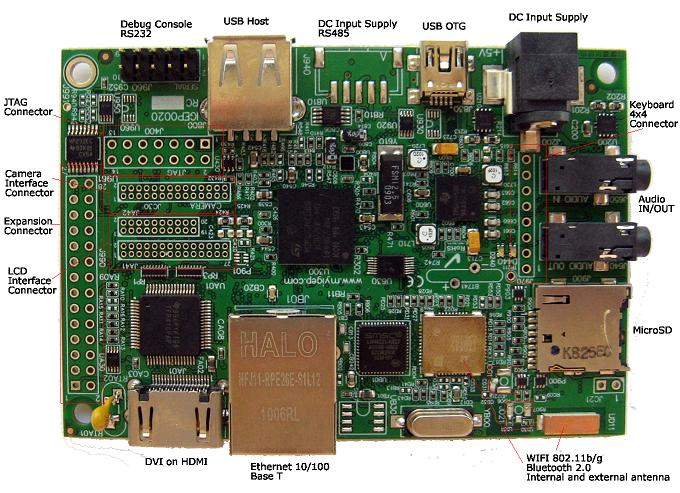
\includegraphics[width=\textwidth]{afbeeldingen/IGEPv2}
	\caption{IGEPv2}
\end{figure}

Dat hebben we gevonden in de vorm van de \strong{\makeurl{http://www.globalscaletechnologies.com/t-guruplugdisplaydetails.aspx}{GuruPlug Display}}. Deze computer is misschien minder krachtig (vooral acceleratiemogelijkheden zijn een prominente afwezige), maar wordt geleverd als een sluitend geheel waarbij het standaardpakket tevens voorziet van alle nodige kabels.

\begin{figure}
	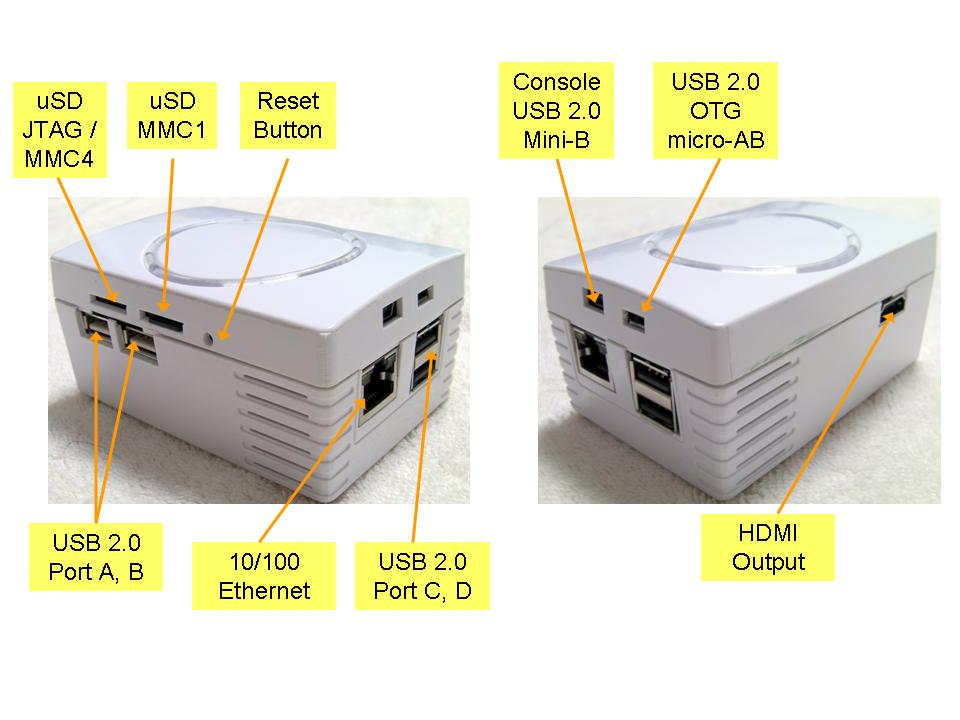
\includegraphics[width=\textwidth]{afbeeldingen/GuruPlug_Display}
	\caption{GuruPlug Display}
\end{figure}

Verschillende maanden hebben we dan ook gedacht dat we de GuruPlug Display zouden gebruiken, meer nog: we waren reeds begonnen met de ontwikkeling van een besturingssysteem voor deze hardware. Er doken echter problemen op toen we tot aankoop van de hardware wouden overgaan. Vooreerst werd bij aankoop van een enkel device ter ontwikkeling van het besturingssysteem meer dan \euro 40 aan portkosten aangerekend, wat een significante meerkost betekende. Vervolgens liet het bedrijf achter de GuruPlugs weten dat er geen Europese modellen zouden gemaakt worden, waardoor we tevens een conversiestekker zouden moeten aankopen. Aangezien de hardware reeds niet al te performant was, hebben we wegens deze twee meerkosten besloten om opnieuw uit te gaan kijken naar een alternatieve oplossing, ondanks het feit dat we al begonnen waren met de effectieve implementatie.

Daarom zijn we op zoek gegaan naar een vergelijkbare plug-computer (zodat we niet veel werk zouden moeten herdoen), die beter leverbaar is, en dat liefst ook binnen Europa. Zo zijn we gestuit op de \strong{\makeurl{http://www.genesi-usa.com/products/efika}{EFIKA MX}} Smarttop computer, een computer vergelijkbaar met de GuruPlug. Meer zelfs, bepaalde elementen (zoals de \ac{cpu} generatie en de \ac{gpu}) hebben zelfs betere specificaties. Daartegenover staat dat er geen Bluetooth aanwezig is, alsook de prijs ietwat hoger ligt. Maar omdat Genesis een verdeler in het Verenigd Koninkrijk heeft, verdwijnt die meerkost daar we geen portkosten moeten betalen bij de uiteindelijke bestelling.

\begin{figure}
	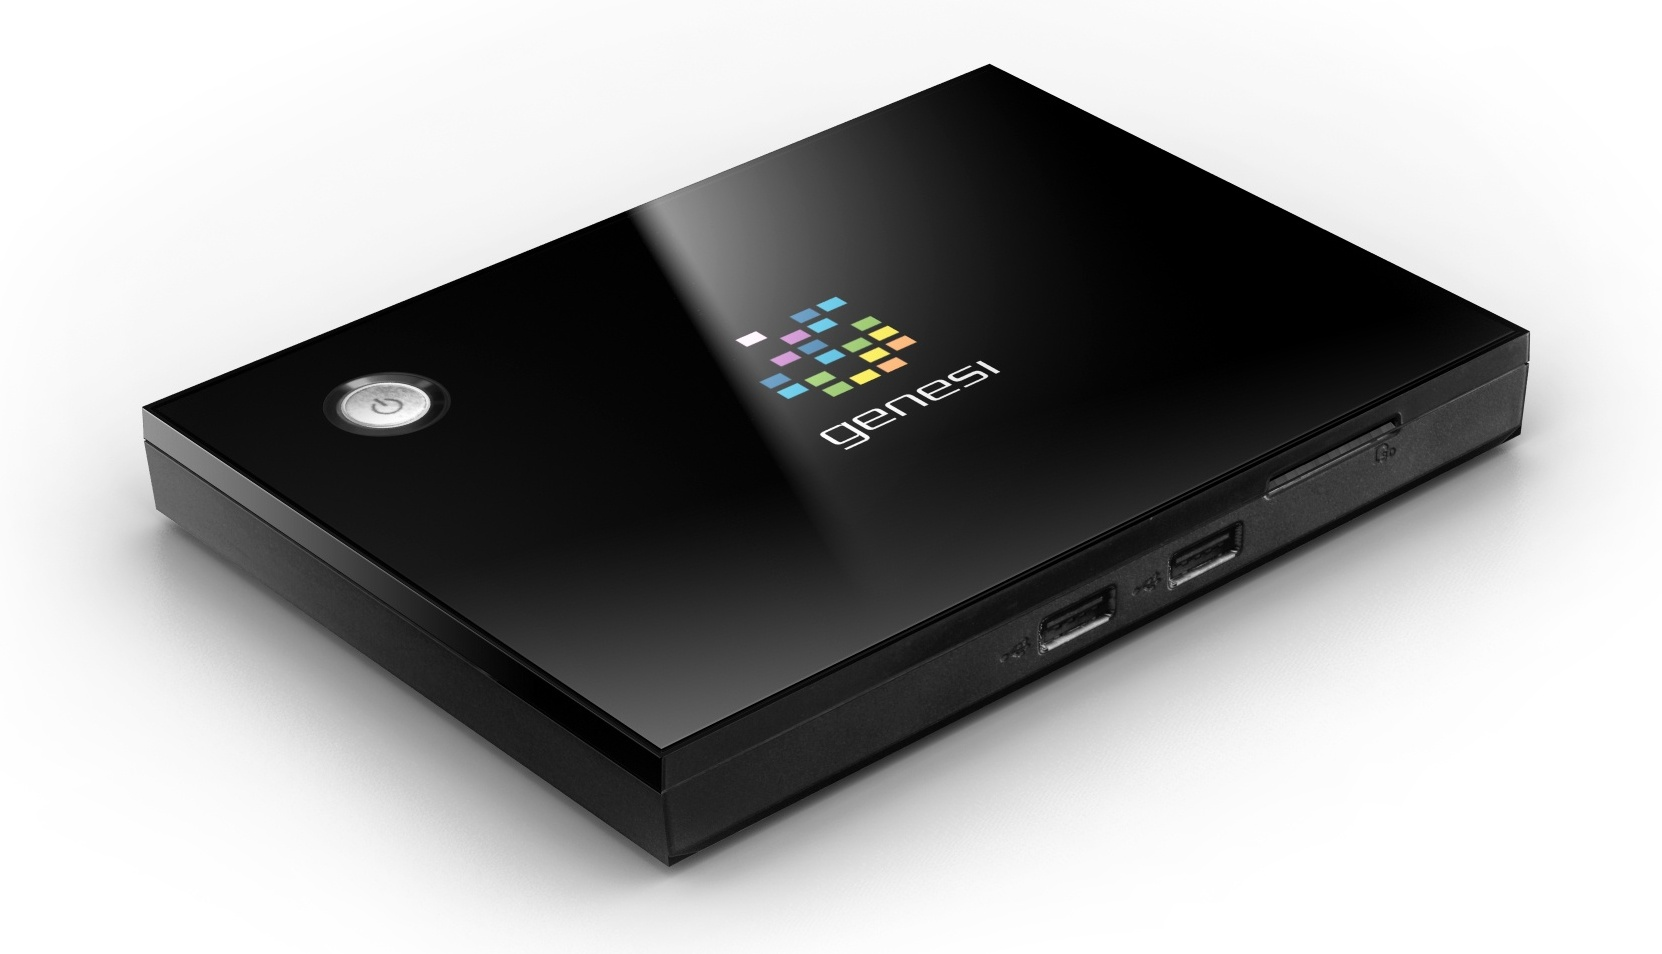
\includegraphics[width=\textwidth]{afbeeldingen/EFIKA_MX}
	\caption{Genesis EFIKA MX}
\end{figure}

\section{Input module}
\label{ontwerp:hardware:input}

De gebruikersinterface wordt gerealiseerd door 4 grote drukknoppen ingebouwd in de kast van elke kiosk. Momenteel worden deze knoppen intern doorverbonden met een afstandsbediening, waardoor de gebruiker via het indrukken van de knoppen indirect de DVD-speler kan besturen om zo een fragment te selecteren.

\begin{figure}
	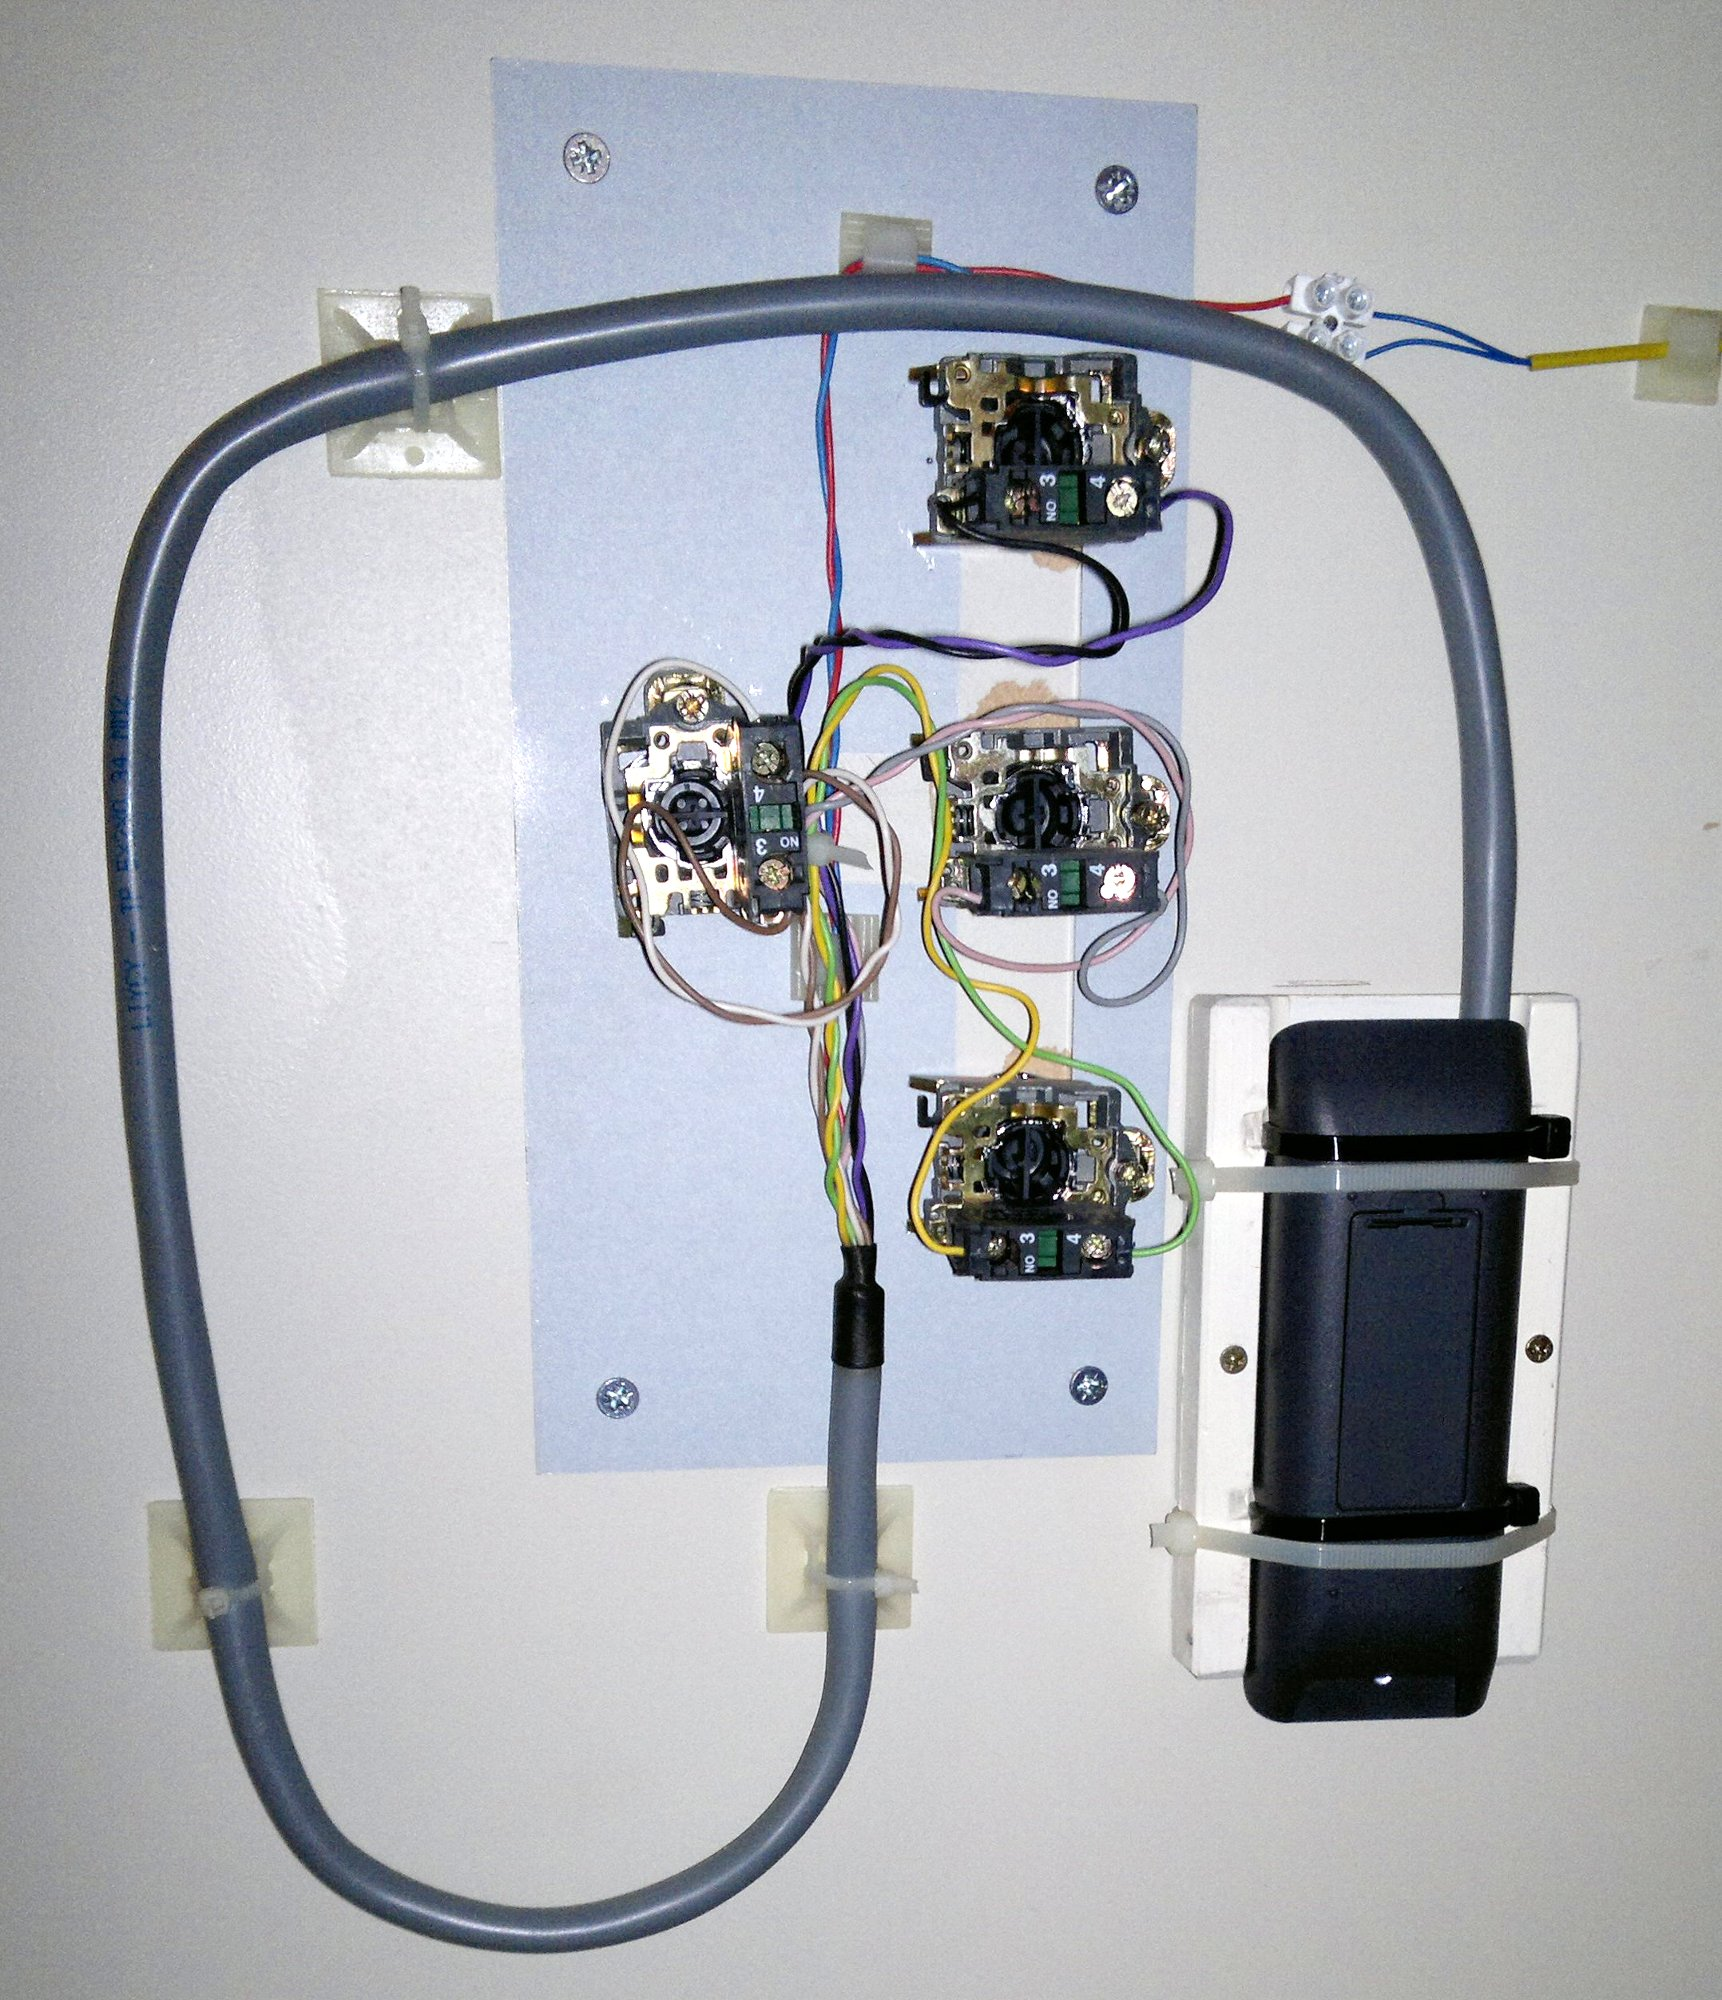
\includegraphics[width=\textwidth]{afbeeldingen/kiosk_knoppen}
	\caption{Huidige aansluitingsmethode knoppen}
\end{figure}

Nu we echter de DVD-spelers gaan vervangen door een computer, zullen we ook voor deze input module een compatibel alternatief moeten vinden. Aan deze module worden enkele specifieke eisen gesteld:
\begin{itemize}
\item Goedkoop: de module moet zo goedkoop mogelijk te produceren zijn, alsook mag het niet teveel energie verbruiken;
\item Toekomstgericht: aansluitmogelijkheden mogen geen gebruik maken van oude protocollen;
\item Gebruiksvriendelijk: installatie van de module moet eenvoudig zijn;
\item Snel: de tijd tussen het indrukken van een toets en registratie van het signaal moet minimaal zijn;
\item Uitbreidbaar: het moet mogelijk zijn om later extra toetsen aan te sluiten.
\end{itemize}

\subsection{Aansluiting}

Het grootste ontwerpprobleem hierbij is de manier van aansluiting die we zullen gebruiken om de module in verbinding te brengen met de rest van de kioskhardware. De meeste eenvoudige keuze zou die zijn van de \strong{parallelle poort}, waarbij we de pinnen van de poort vrijwel direct zouden kunnen verbinden met de knoppen. Jammer genoeg zijn parallelle poorten steeds schaarser, en komt die vrijwel nooit meer voor op embedded hardware. Een andere toegankelijke optie is de \strong{seriële poort}. Hierbij zou dan extra periferie benodigd zijn om in te staan voor de serialisatie van de signalen. Indien we echter platform-specifieke code toelaten, kunnen we de stuursignalen van de poort op een parallelle manier misbruiken zodat ook die periferie geëlimineerd wordt. Toch voldoet ook deze oplossing niet: ook de seriële poort wordt steeds schaarser, en alhoewel ze momenteel nog te vinden is op de meeste embedded-hardware bestaat de mogelijkheid dat dit binnen geringe tijd niet meer zo is.

Daarom hebben we uiteindelijk gekozen voor een poort die we normaal gezien wel nog enkele jaren zullen terugvinden op de meest courante hardware: de \ac{usb} poort. Deze veelzijdige poort laat ons doe om de input module te laten communiceren met een computer, en is ook relatief toekomstgericht (de recent geïntroduceerde \ac{usb} versie 3 is nog steeds volledig terugwaarts compatibel met \ac{usb} versie 1 toestellen). Maar het gebruik van \ac{usb} kent ook een nadeel: het protocol is immers pakket-georiënteerd, waardoor extra periferie een noodzaak is. Ook is de configuratie complexer, zeker indien we een toestel willen dat zonder speciale stuurprogramma's werkt op verschillende besturingssystemen.

\subsection{Realisatie \acs{usb}-communicatie}

Aangezien \ac{usb} een pakket-georiënteerd protocol is, hebben we steeds extra periferie nodig om de gebruikersinvoer door te sturen. Om geen speciale software te vereisen moet onze module een apparaat uit de \ac{usb} \ac{hid} klasse implementeren. Voor bepaalde subcategorieën van deze klasse (zoals toetsenborden, muizen, \dots) wordt immers gegarandeerd dat compatibele besturingssystemen er mee zullen kunnen omgaan zonder daarvoor extra stuurprogramma's nodig te hebben. Daarom zullen we onze module zichzelf laten identificeren als een toetsenbord, waarbij we dan in de Javascript code van de voorstellingen gepast kunnen reageren op dergelijke toetsaanslagen.

Om een \ac{usb} toetsenbord te realiseren, zijn we in eerste instantie op zoek gegaan naar \strong{\ac{usb} keyboard encoders}. In de huidige opzet hebben we echter maar nood aan 4 knoppen, terwijl de meeste keyboard encoders veel meer toetsen toelaten. Daarom is de prijs meestal ook een pak hoger, zo kost de \makeurl{http://www.ultimarc.com/ipacve.html}{I-Pac VE} keyboard encoder, die 32 toetsen toelaat, reeds \$35!

Daarom lijkt het interessanter om zelf te voorzien in de conversie naar \ac{usb}-pakketten, door gebruik te maken van een \strong{microcontroller met \ac{usb} hardware}. Dergelijke microcontrollers voorzien in on-chip \ac{usb} communicatiemogelijkheden, net zoals de meeste reguliere microcontrollers toelaten om gegevens over een seriële \ac{uart} te transporteren. Om vervolgens de \ac{usb} hardware op een toegankelijke manier te gebruiken, bestaan er verschillende bibliotheken zoals de officiële \ac{usb} bibliotheek van Atmel, of het open-source \makeurl{http://www.fourwalledcubicle.com/LUFA.php}{\ac{lufa}}. Het nadeel van deze piste is echter de meerkost van de \ac{usb} hardware, die eigenlijk onnodig is daar we enkel gebruik zullen maken van de \emph{low speed} overdrachtsmodus.

Een derde optie is om gebruik te maken van een \strong{microcontroller met \ac{usb} software}. Hierbij hebben we geen speciale hardware nodig, enkel een microcontroller die krachtig genoeg is om de \ac{usb} software uit te voeren. Het grote nadeel hieraan is dat het met de huidige microcontrollers enkel mogelijk is om gebruik te maken van \emph{low speed} \ac{usb}, maar voor onze toepassing is dit geen probleem. Opnieuw zijn er verschillende mogelijkheden om dit te realiseren, waarvan er een beschreven is in een \makeurl{http://www.atmel.com/dyn/resources/prod\_documents/doc2556.pdf}{application note} van Atmel. Deze application note gebruikt relatief weinig hardware om elementaire \ac{usb} communicatie te realiseren, maar zoals later zal blijken zijn er zelfs nog efficiëntere configuraties mogelijk. Ook is de software geschreven in AVR assembler, waardoor het geheel niet zo overdraagbaar is. Daarom zullen we gebruik maken van een open-source alternatief: de \makeurl{http://www.obdev.at/products/vusb/index.html}{V-USB} bibliotheek. Deze in C-geschreven bibliotheek biedt een eenvoudigere interface en daarbij ook verschillende voorbeeldprojecten om het gebruik ervan te illustreren.


%
% Licenties
%

\chapter{Licenties}

Bij de keuze van codebibliotheken en technologieën hebben we vaak rekening gehouden met overdraagbaarheid en platform-onafhankelijkheid zodat het steeds mogelijk blijft om de ontwikkelde software eventueel te gebruiken in andere musea en daar zelf eventueel munt uit te slaan.

% licentie hardware: cern

% licentie thesis: cc by

